% Title page
\frame[plain]{\titlepage}

\lecture{Введение}{intro}

\section{Факты, правила и запросы}
\subsection{Основные пункты}

\begin{frame}
	\frametitle{\insertsection}
	\framesubtitle{\insertsubsection}
	\begin{itemize}
		\item Рассмотреть простые примеры программ на \textbf{Prolog}, определить понятия факта, правила, запроса и базы знаний
		\item Дать определения основных понятий и синтаксических конструкций, таких как атомы, переменные и термы
	\end{itemize}
\end{frame}

\subsection{База знаний}

\begin{frame}
	\frametitle{\insertsection}
	\framesubtitle{\insertsubsection}
	Базовые конструкции языка \textbf{Prolog}:
	\begin{itemize}
		\item Факты
		\item Правила
		\item Запросы
	\end{itemize}
	Программа на Prolog представляет собой множество \textbf{фактов} и \textbf{правил}~--- \alert{Базу Знаний}
	Чтобы использовать информацию, содержащуюся в базе знаний, необходимо ставить \textbf{запросы}.
\end{frame}

\begin{frame}
	\frametitle{\insertsection}
	\framesubtitle{\insertsubsection}
	Пример 1
	
	
	\texttt{\begin{itemize}
				\item[] woman(mia).
				\item[] woman(jody).
				\item[] woman(yolanda).
				\item[] playsGuitar(jody).
				\item[]<2-> listensToMusic(mia).
				\item[]<2-> musician(yolanda).
				\item[]<2-> playsGuitar(mia) :- listensToMusic(mia).
				\item[]<2-> playsGuitar(yolanda) :- listensToMusic(yolanda).
				\item[]<2-> listensToMusic(yolanda) :- musician(yolanda).
			\end{itemize}}
\end{frame}

\begin{frame}
	\frametitle{\insertsection}
	\framesubtitle{\insertsubsection}
	Пример 2
	
	
	\texttt{\begin{itemize}
		\item[] musician(mia).
		\item[] listensToMusic(jody).
		\item[] playsGuitar(mia) :- listensToMusic(mia),musician(mia).
		\item[] playsGuitar(jody) :- musician(jody); listensToMusic(jody).
	\end{itemize}}
\end{frame}

\begin{frame}
	\frametitle{\insertsection}
	\framesubtitle{\insertsubsection}
	Пример 3
	
	
	\texttt{\begin{itemize}
		\item[] woman(mia).
		\item[] woman(jody).
		\item[] woman(yolanda).
		\item[] loves(vincent,mia).
		\item[] loves(marcellus,mia).
	\end{itemize}}
\end{frame}

\begin{frame}
	\frametitle{\insertsection}
	\framesubtitle{\insertsubsection}
	Пример 4
	
	
	\texttt{\begin{itemize}
			\item[] loves(vincent,mia).
			\item[] loves(marcellus,mia).
			\item[] jealous(X,Y) :- loves(X,Z),loves(Y,Z).
	\end{itemize}}
\end{frame}

\subsection{Синтаксис}

\begin{frame}
	\frametitle{\insertsection}
	\framesubtitle{\insertsubsection}
	\textbf{\underline{Атомы}}
	
	\begin{enumerate}
		\item Последовательность строчных или прописных букв, цифр и символов подчерка, начинающаяся со строчной буквы.
		\item Произвольная последовательность символов, заключённая в одинарные кавычки.
		\item Последовательность спецсимволов.
	\end{enumerate}

	\begin{rexample}
		mia, marcellus, big\_kahuna\_burger, 'Произвольная строка символов', ====>, :-
	\end{rexample}
\end{frame}

\begin{frame}
	\frametitle{\insertsection}
	\framesubtitle{\insertsubsection}
	\textbf{\underline{Числа}}
	
	\begin{enumerate}
		\item Действительные числа: 2,718; 103,3087; \(\pi \), \ldots
		\item Целые числа: -2, -1, 0, 1, 2, \ldots
	\end{enumerate}

	\textbf{\underline{Переменные}}
	
	
	\textbf{Переменные} служат для обозначения объектов, значения которых меняются в ходе выполнения программы. Имя переменной задается
	последовательностью строчных или прописных букв, цифр и символов подчерка, начинающейся с \textbf{прописной буквы} или \textbf{символа подчерка}.
	
	\begin{rexample}
		X, Y, Variable, \_X, X1, \_variable\_with\_some\_info\_
	\end{rexample}
\end{frame}

\begin{frame}
	\frametitle{\insertsection}
	\framesubtitle{\insertsubsection}
	\textbf{\underline{Термы}}
	
	\textit{Терм (составной терм)} состоит из \alert{функтора} и последовательности аргументов в скобках.
	\begin{enumerate}
		\item Любой атом или число является термом. Такие термы называются \alert{константами}.
		\item Любая переменная является термом.
		\item Имя функтора~--- это атом.
		\item Переменная не может быть функтором.
		\item Аргументы составного терма должны быть термами.
	\end{enumerate}

	\begin{rexample}
		loves(vincent, mia), playsGuitar(jody), jody, musician(mia), eats(cat,Prey)
	\end{rexample}
\end{frame}

\subsection{Проверочные вопросы}

\begin{frame}
	\frametitle{\insertsection}
	\framesubtitle{\insertsubsection}
	Какие из перечисленных строк являются атомами, какие переменными, а какие не являются ни тем, ни другим?
	\texttt{\begin{enumerate}
		\item vINCENT
		\item Foot
		\item x1
		\item Y3
		\item big\_kahuna\_burger
		\item 'Криминальное чтиво'
		\item roast chicken
		\item \_IndianaJones
		\item '\_IndianaJones'
	\end{enumerate}}
\end{frame}

\begin{frame}
	\frametitle{\insertsection}
	\framesubtitle{\insertsubsection}
	Какие из перечисленных ниже строк являются атомами, переменными или составными термами, а какие вообще не являются термами? Для каждого составного терма укажите имя функтора и его арность.
	\texttt{\begin{enumerate}
		\item loves(vincent,mia)
		\item 'loves(vincent,mia)'
		\item Eats(cat,mouse)
		\item hasChildren(cat,kittens)
		\item and(musician(jody),artist(mia))
		\item and(musician(X),artist(Y))
		\item \_and(musician(jody),artist(mia))
		\item (Butch kills Vincent)
		\item kills(Butch,Vincent)
		\item kills(Butch,Vincent
	\end{enumerate}}
\end{frame}

\begin{frame}
	\frametitle{\insertsection}
	\framesubtitle{\insertsubsection}
	Сколько фактов, правил, высказываний и предикатов в следующей базе знаний? Для каждого правила назовите вывод и цели.
	\texttt{\begin{itemize}
			\item[] woman(mia).
			\item[] woman(jody).
			\item[] man(jules).
			\item[] person(X) :- man(X); woman(X).
			\item[] loves(X,Y) :- knows(Y,X).
			\item[] father(Y,Z) :- man(Y), son(Z,Y).
			\item[] father(Y,Z) :- man(Y), daughter(Z,Y).
	\end{itemize}}
\end{frame}

\subsection{Упражнения}

\begin{frame}
	\frametitle{\insertsection}
	\framesubtitle{\insertsubsection}
	Запишите следующую базу знаний на языке Prolog.
	
	\begin{itemize}
		\item Бутч убийца.
		\item Миа и Марселлас женаты.
		\item Зед мертв.
		\item Марселлас убьет любого, кто сделает Мие массаж стопы.
		\item Миа любит любого, кто хорошо танцует.
		\item Джулс ест все, что вкусно или питательно.
	\end{itemize}
\end{frame}

\begin{frame}
	\frametitle{\insertsection}
	\framesubtitle{\insertsubsection}
	Пусть дана следующая база знаний:
	\texttt{\begin{itemize}
			\item[] sportsman(john).
			\item[] hasUniform(harry).
			\item[] footballPlayer(harry).
			\item[] sportsman(X) :- isTrained(X),hasUniform(X).
			\item[] isTrained(X) :- footballPlayer(X).
	\end{itemize}}
	
	Как Prolog ответит на следующие запросы?
	\texttt{\begin{enumerate}
			\item sportsman(john).
			\item footballPlayer(john).
			\item sportsman(harry).
			\item sportsman(X).
			\item hockeyPlayer(john).
	\end{enumerate}}
\end{frame}

\subsection{Дополнительное задание}

\begin{frame}
	\frametitle{\insertsection}
	\framesubtitle{\insertsubsection}
	Средствами языка Prolog \textbf{определить, какие животные не имеют хозяина.}
	\begin{enumerate}
		\item Бутси~--- коричневая кошка.
		\item Корни~--- черная кошка.
		\item Мак~--- рыжая кошка.
		\item Флэш, Ровер и Спот~--- собаки, Ровер~--- рыжая, а Спот~--- белая.
		\item Все животные, которыми владеют Том и Кейт, имеют родословные.
		\item Том владеет всеми черными и коричневыми животными, а Кейт владеет всеми собаками небелого цвета, которые не являются собственностью Тома.
		\item Алан владеет Мак, если Кейт не владеет Бутси и если Спот не имеет родословной.
		\item Флэш~--- пятнистая собака.
	\end{enumerate}
\end{frame}

\lecture{Matching}{match}

\section{Унификация термов и поиск решений}
\subsection{Основные пункты}

\begin{frame}
	\frametitle{\insertsection}
	\framesubtitle{\insertsubsection}
	\begin{itemize}
		\item Познакомиться с понятием согласования термов.
		\item Разобраться в стратегиях, используемых интерпретатором языка Prolog для поиска ответов на вопросы.
	\end{itemize}
\end{frame}

\subsection{Определение}

\begin{frame}
	\frametitle{\insertsection}
	\framesubtitle{\insertsubsection}
	\only<1>{Два терма \alert{унифицированы}, если они равны или если они содержат переменные и существует означивание этих переменных, такое, что термы становятся равными.}
	\only<2->{\begin{enumerate}
			\item Если \texttt{term1} и \texttt{term2} константы, то \texttt{term1} и \texttt{term2} унифицированы тогда и только тогда, когда они равны друг другу, т.е. \texttt{term1} и \texttt{term2} это один и тот же атом или число.
			\item Если \texttt{term1}~--- это переменная, а \texttt{term2}~--- любой терм, то термы \texttt{term1} и \texttt{term2} унифицированы, и переменная \texttt{term1} инициализируется значением терма \texttt{term2}. 
			Если \texttt{term1} и \texttt{term2}~--- переменные, они унифицированы и принимают значения друг друга. Говорят, что переменные \texttt{term1} и \texttt{term2} \alert{разделяют значение}.
			\item Если \texttt{term1} и \texttt{term2} составные термы, то они унифицированы тогда и только тогда, когда:
			\begin{enumerate}[(a)]
				\item Их функторы и арность совпадают.
				\item Соответствующие аргументы обоих термов унифицированы. При этом означивание переменных согласовано.
			\end{enumerate}
			\item Два терма унифицированы тогда и только тогда, когда это следует из одного из предыдущих пунктов.
	\end{enumerate}}
\end{frame}

\subsection{Примеры унификации}

\begin{frame}
	\frametitle{\insertsection}
	\framesubtitle{\insertsubsection}
	\textbf{Какие из термов унифицированы?}
	\texttt{\begin{itemize}
		\item john = john.
		\item 42 = 42.
		\item 'Строка слов' = 'Строка слов'.
		\item 'mia' = mia.
		\item '42' = 42.
		\item mia = X.
		\item X = Y.
		\item kill(shoot(gun),Y) = kill(X,stab(knife)).
		\item loves(X,X) = loves(marcellus,mia).
		\item parent(A) = A.
	\end{itemize}}
\end{frame}

\subsection{Поиск решений}

\begin{frame}
	\frametitle{\insertsection}
	\framesubtitle{\insertsubsection}
	Интерпретатор языка Prolog обрабатывает условия запроса последовательно слева направо. Для каждого из условий интерпретатор ищет унифицируемый с ним факт или вывод правила, проходя базу знаний сверху вниз.
\end{frame}

\begin{frame}
	\frametitle{\insertsection}
	\framesubtitle{\insertsubsection}
	\texttt{\begin{itemize}
			\item[] person(vincent).
			\item[] person(jules).
			\item[] hasGun(vincent).
			\item[] hasGun(jules).
			\item[] alive(jules).
			\item[] lucky(X) :- person(X),hasGun(X),alive(X).
	\end{itemize}}
\end{frame}

\subsection{Дерево поиска решений}

\begin{frame}
	\frametitle{\insertsection}
	\framesubtitle{\insertsubsection}
	\begin{figure}
		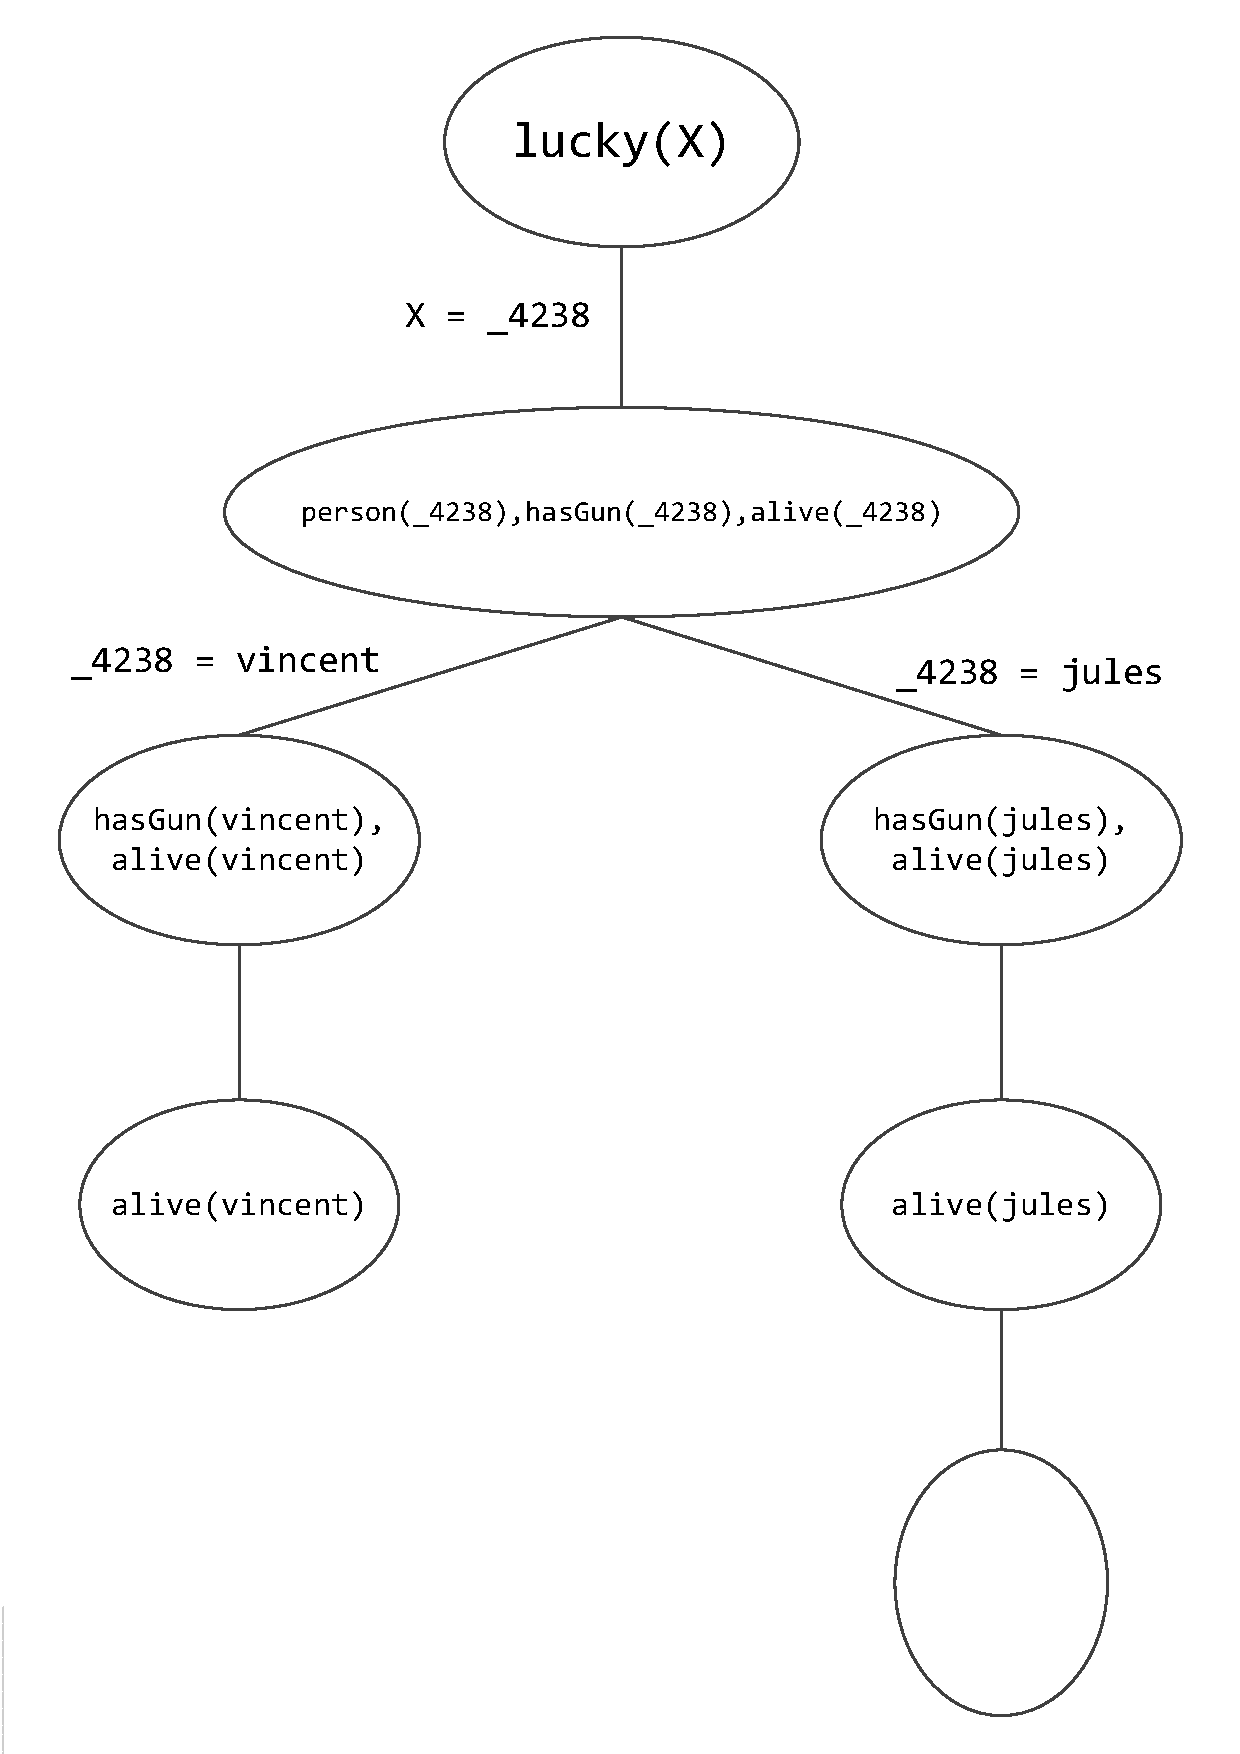
\includegraphics[scale=0.35]{stree}
	\end{figure}
\end{frame}

\subsection{Упражнения}

\begin{frame}
	\frametitle{\insertsection}
	\framesubtitle{\insertsubsection}
	В каких из перечисленных пар термы унифицированы? Где необходимо запишите значения переменных, необходимые для унификации.
	\texttt{\begin{enumerate}
			\item bread = bread.
			\item 'Bread' = bread.
			\item 'bread' = bread.
			\item Bread = bread.
			\item хлеб = котлета.
			\item food(bread) = bread.
			\item food(bread) = Bread.
			\item food(Bread) = food(bread).
			\item food(хлеб,X) = food(Y,котлета).
			\item graph(edge(v1,v2),X,edge(Y,v4)) = graph(Z,edge(v7,v8),edge(v4,X)).
			\item food(X) = X.
			\item meal(food(bread),drink(beer)) = meal(food(X),Y).
			\item meal(food(bread),X) = meal(X,drink(beer)).
	\end{enumerate}}
\end{frame}

\begin{frame}
	\frametitle{\insertsection}
	\framesubtitle{\insertsubsection}
	\textbf{Пусть дана следующая база знаний.}
	\texttt{\begin{itemize}
			\item[] witch(gullveig).
			\item[] god(freyja).
			\item[] god(odin).
			\item[] god('Vidarr').
			\item[] magic(X) :- witch(X).
			\item[] magic(X) :- wizard(X).
			\item[] magic(X) :- god(X).
	\end{itemize}}
	\textbf{Каким из запросов она удовлетворяет?}
	\texttt{\begin{enumerate}
			\item magic(witch).
			\item wizard(odin).
			\item magic('Vidarr').
			\item magic(Vidarr).
	\end{enumerate}}
\end{frame}

\begin{frame}
	\frametitle{\insertsection}
	\framesubtitle{\insertsubsection}
	\textbf{Дан следующий лексикон.}
	\texttt{\begin{itemize}
			\item[] word(article,a).
			\item[] word(article,every).
			\item[] word(noun,criminal).
			\item[] word(noun,'big kahuna burger').
			\item[] word(verb,eats).
			\item[] word(verb,likes).
%			\item[] sentence(W1,W2,W3,W4,W5) :- word(article,W1), word(noun,W2), word(verb,W3), word(article,W4), word(noun,W5).
	\end{itemize}}
	Написать запрос на получение списка всех возможных фраз данного лексикона, имеющих вид: \textit{артикль+существительное+глагол+артикль+существительное}. Построить дерево поиска решений для одной из построенных фраз.
\end{frame}

\begin{frame}
	\frametitle{\insertsection}
	\framesubtitle{\insertsubsection}
	Имеется следующий список слов: \textit{бок, акр, сомо, бокс, хата, эдда, вино, рода, окот, анод, скала, онагр, обиход, монако, дверка, дигора, удокан, маарри, бинокль, бегония}.
	Пусть в базе знаний слова представляются следующим образом:
	\texttt{\begin{itemize}
			\item[] word(эдда,э,д,д,а).
			\item[] word(вино,в,и,н,о).
			\item[] word(рода,р,о,д,а).
			\item[] word(окот,о,к,о,т).
			\item[] word(анод,а,н,о,д).
			\item[] word(скала,с,к,а,л,а).
			\item[] word(онагр,о,н,а,г,р).
			\item[] word(обиход,о,б,и,х,о,д).
	\end{itemize}}
\end{frame}

\begin{frame}
	\frametitle{\insertsection}
	\framesubtitle{\insertsubsection}
	Реализовать предикат \texttt{crosswd/10 = crosswd(V1,V2,V3,V4,V5,V6,H1,H2,H3,H4)}, который бы заполнял данными словами следующий кроссворд таким образом, чтобы
	слова, идущие вертикально, были первыми 6 аргументами, а слова, идущие горизонтально~--- последними.
	\begin{figure}
		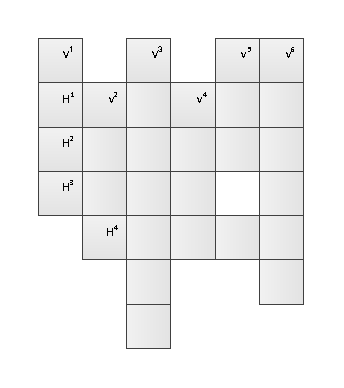
\includegraphics[scale=0.9]{crosswd}
	\end{figure}
\end{frame}

\lecture{Recursion}{recursion}

\begin{frame}[plain,c]

	\begin{center}
		\Huge Определения и примеры
	\end{center}

\end{frame}

\section{Рекурсия в Prolog}
\subsection{Простой пример}

\begin{frame}
	\frametitle{\insertsection}
	\framesubtitle{\insertsubsection}
	\texttt{\begin{itemize}
			\item[] переваривает(Хищник,Добыча) :- съел(Хищник,Добыча).
			\item[] переваривает(Хищник,Добыча) :- съел(Хищник,ДругойХищник), переваривает(ДругойХищник,Добыча).
			\item[] съел(комар,кровь).
			\item[] съел(лягушка, комар).
			\item[] съел(цапля, лягушка).
	\end{itemize}}
\end{frame}

\section{Уровни понимания программ}
\subsection{Декларативный и процедурный}

\begin{frame}
	\frametitle{\insertsection}
	\framesubtitle{\insertsubsection}
	\alert{Декларативный смысл} Prolog-программы касается только \textit{отношений}, определенных в программе.
	Другими словами, декларативный смысл определяет, что должно быть результатом работы программы с точки зрения математической логики.
	
	\alert{Процедурный смысл} программы определяет еще и как этот результат был получен, т.е. как отношения реально обрабатываются пролог-системой.
\end{frame}

\section{Правила описания рекурсивных предикатов}
\subsection{База и шаг рекурсии}

\begin{frame}
	\frametitle{\insertsection}
	\framesubtitle{\insertsubsection}
	\only<1>{\textbf{База рекурсии}}
	\only<2>{\textbf{Шаг рекурсии}}
	
	
	\texttt{\begin{itemize}
			\item[] {\color<1>[RGB]{0,0,255}{переваривает(Хищник,Добыча) :- съел(Хищник,Добыча).}}
			\item[] {\color<2>[RGB]{0,0,255}{переваривает(Хищник,Добыча) :- съел(Хищник,ДругойХищник), переваривает(ДругойХищник,Добыча).}}
			\item[] съел(комар,кровь).
			\item[] съел(лягушка, комар).
			\item[] съел(цапля, лягушка).
	\end{itemize}}
\end{frame}

\subsection{descending.pl}

\begin{frame}
	\frametitle{\insertsection}
	\framesubtitle{\insertsubsection}
	\texttt{\begin{itemize}
			\item[] child(adam,cain).
			\item[] child(adam,abel).
			\item[] child(adam,seth).
			\item[] child(cain,enoch).
			\item[] child(enoch,irad).
			\item[] child(irad,mehujael).
			\item[] child(seth,enos).
			\item[] child(enos,kenan).
			\item[] child(kenan,mahalalel).
			\item<2->[] descend(A,D) :- child(A,D).
			\item<2->[] descend(A,D) :- child(A,C), descend(C,D).
	\end{itemize}}
\end{frame}

\subsection{arithmetic.pl}

\begin{frame}
	\frametitle{\insertsection}
	\framesubtitle{\insertsubsection}
	\texttt{\begin{itemize}
			\item[] num(0).
			\item[] num(s(N)) :- num(N).
			\item<2->[] plus(0,N,N).
			\item<2->[] plus(s(M),N,s(Sum)) :- plus(M,N,Sum).
	\end{itemize}}
\end{frame}

\section{Рекурсия и хвостовая рекурсия}
\subsection{Численная арифметика: вычисление факториала числа}

\begin{frame}
	\frametitle{\insertsection}
	\framesubtitle{\insertsubsection}
	
	\texttt{\begin{itemize}
			\item[] f(0,1).
			\item[] f(X,Y) :- X>0,X1 is X-1,f(X1,Y1),Y is Y1*X.
	\end{itemize}}

	\uncover<2->{\texttt{\begin{itemize}
				\item[] f(N,N,F):-write(F),!.
				\item[] f(N,N1,F1):- N2 is N1+1,F2 is F1*N2,f(N,N2,F2).
				\item[] factorial(N):- f(N,1,1).
	\end{itemize}}}

\end{frame}

\section{Последовательность целей и остановка программ}
\subsection{Возможные источники ошибок}

\begin{frame}

	\frametitle{\insertsection}
	\framesubtitle{\insertsubsection}
	\texttt{\begin{itemize}
			\item[] child(adam,cain).
			\item[] child(adam,abel).
			\item[] child(adam,seth).
			\item[] child(cain,enoch).
			\item[] child(enoch,irad).
			\item[] child(irad,mehujael).
			\item[] child(seth,enos).
			\item[] child(enos,kenan).
			\item[] child(kenan,mahalalel).
	\end{itemize}}
	\texttt{\only<1>{\begin{itemize}
				\item[] descend(A,D) :- child(A,D).
				\item[] descend(A,D) :- child(A,C), descend(C,D).
			\end{itemize}}
		\only<2>{\begin{itemize}
				\item[] descend(A,D) :- descend(C,D), child(A,C).
				\item[] descend(A,D) :- child(A,D).
		\end{itemize}}
		\only<3>{\begin{itemize}
				\item[] descend(A,D) :- child(A,D).
				\item[] descend(A,D) :- descend(C,D), child(A,C).
		\end{itemize}}
		\only<4>{\begin{itemize}
				\item[] descend(A,D) :- child(A,C), descend(C,D).
				\item[] descend(A,D) :- child(A,D).
		\end{itemize}}
	}

\end{frame}

\begin{frame}

	\frametitle{\insertsection}
	\framesubtitle{\insertsubsection}
	
	\texttt{\begin{itemize}
			\item[] num(0).
			\item[] num(s(N)) :- num(N).
		\end{itemize}
	}
	
	\texttt{\begin{itemize}
			\item[] num(s(N)) :- num(N).
			\item[] num(0).
		\end{itemize}
	}

\end{frame}

\begin{frame}[plain,c]

	\begin{center}
		\Huge Упражнения
	\end{center}

\end{frame}


\section{Упражнения}

\begin{frame}
	\frametitle{\insertsection}
	\begin{itemize}
		\item Скачайте или перепишите листинг программы \texttt{descending.pl}. Рассмотрите каждый случай рекурсии (см. слайды ранее). Какие запросы работают, какие нет? Почему?
		\item Скачайте или перепишите листинг программы \texttt{arithmetic.pl}. Реализуйте следующие операции над числами, определенными в программе:
		\begin{enumerate}
			\item \textbf{Умножение}: реализуйте предикат \texttt{times/3}, такой, чтобы последним аргументом было произведение двух первых.
			\item \textbf{Возведение в степень}: реализуйте предикат \texttt{exp(N,X,R)}, такой, чтобы \(R = X^{N}\).
			\item \textbf{Сравнение}: реализуйте предикаты \texttt{gt/2, lt/2}, истинные тогда, когда первый аргумент больше (меньше), чем второй.
			\item \textbf{Равенство}: реализуйте предикат \texttt{eq/2}, истинный тогда и только тогда, когда его аргументы равны.
			\item \textbf{Максимум и минимум двух чисел}: реализуйте предикаты \texttt{max/3, min/3}, где третий аргумент~--- это максимум (минимум) из двух первых.
		\end{enumerate}
	\end{itemize}
\end{frame}

\begin{frame}
	\frametitle{\insertsection}
	\begin{itemize}
		\item Реализуйте программу для вычисления факториала числа (в обычной численной арифметике). Сравните время работы и количество операций в зависимости от значения входных параметров.
		\item Реализуйте программу для вычисления чисел Фибоначчи. Реализуйте предикат \texttt{getFibN/2 = getFibN(N, Fn)}, такой, что \(F_n\)~--- N-е число Фибоначчи.
		\item Используя предыдущую программу, реализуйте предикат \texttt{getNearestFibonacci/3}, возвращающий по заданному числу номер ближайшего к нему числа Фибоначчи и его номер.
	\end{itemize}
\end{frame}



\lecture{Additional Excercises}{recursionExt}

\section{Дополнительные упражнения}

\begin{frame}
	
	\frametitle{\insertsection}
	
	Преобразуйте программу \texttt{arithmetic.pl}.
	
	\begin{itemize}
		\item Реализуйте операцию деления \(N\) на \(M\) с остатком таким образом, чтобы результатом были два числа \(Q\) и \(P\), такие, что \(N = M\cdot Q + P \).
		\item Реализуйте алгоритм Евклида для поиска наибольшего общего делителя двух заданных чисел.
	\end{itemize}
	
\end{frame}

\begin{frame}
	\frametitle{\insertsection}
	Опишите следующий граф в виде базы знаний. Реализуйте предикат \texttt{fromTo/2 = fromTo(Begin,End)}, который по заданным началу и концу маршрута будет выяснять, существует ли путь между
	заданными вершинами и печатать в консоли слово, которое получается при следовании по найденному пути.
	
	\begin{figure}
		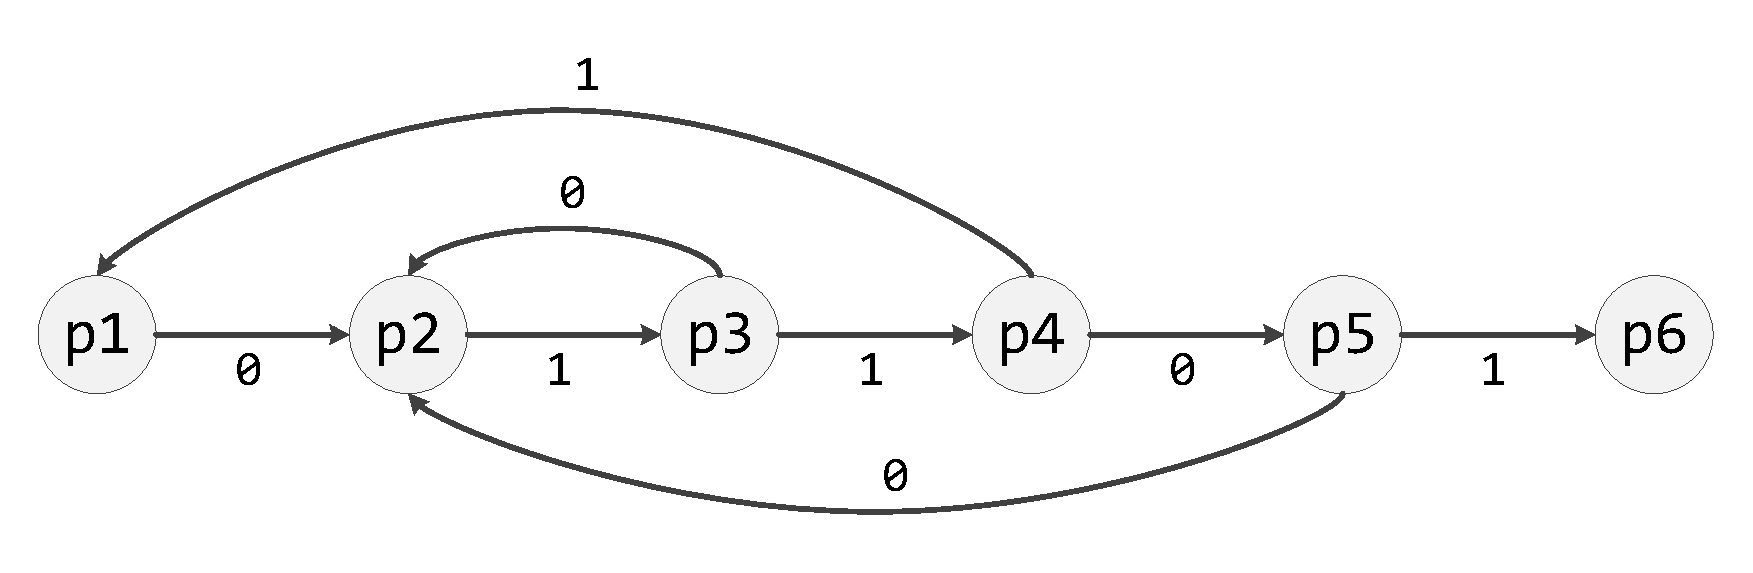
\includegraphics[scale=0.35]{graph}
	\end{figure}
\end{frame}

\begin{frame}[shrink=7]
	\frametitle{\insertsection}
	Скачайте базу знаний \texttt{travel.pl} или перепишите.
	\texttt{\begin{itemize}
		\item[] byCar(auckland,hamilton).
		\item[] byCar(hamilton,raglan).
		\item[] byCar(valmont,saarbruecken).
		\item[] byCar(valmont,metz).
		\item[] byTrain(metz,frankfurt).
		\item[] byTrain(saarbruecken,frankfurt).
		\item[] byTrain(metz,paris).
		\item[] byTrain(saarbruecken,paris).
		\item[] byPlane(frankfurt,bangkok).
		\item[] byPlane(frankfurt,singapore).
		\item[] byPlane(paris,losAngeles).
		\item[] byPlane(bangkok,auckland).
		\item[] byPlane(losAngeles,auckland).
	\end{itemize}}
	Реализуйте предикат \texttt{travel/2}, который по заданным началу и концу маршрута определял бы, существует ли способ добраться из начала в конец и
	печатал пункты маршрута, а также виды транспорта, которыми осуществляется перемещение между промежуточными пунктами.
\end{frame}

\begin{frame}[plain,c]

\begin{center}
	\Huge Домашнее задание
\end{center}

\end{frame}

\section{Домашнее задание}

\begin{frame}
	
	\frametitle{\insertsection}
	
	
	Реализуйте некоторый каталог вида \texttt{unit(key, value)}. Например, список книг по авторам:
	\texttt{\begin{itemize}
			\item[] book(heinlein, 'Stranger in a Strange Land').
			\item[] book(heinlein, 'The Moon Is a Harsh Mistress').
			\item[] book(niven, 'Lucifer's Hammer').
	\end{itemize}}
	
	Реализуйте программу, запрашивающую из консоли ввод автора и печатающую либо список его книг, либо сообщение, что книг данного автора в каталоге нет.
	
	
	\alert{Также на дом остается реализация программы travel.pl с предыдущего слайда, если это не было сделано на занятиях.}
	
\end{frame}


% Списки в Prolog


\lecture{Lists}{lists}

\begin{frame}[plain,c]

	\begin{center}
		\Huge Понятие и вид списка в Prolog
	\end{center}

\end{frame}

\section{Списки}

\subsection{Список в Prolog}

\begin{frame}
	\frametitle{\insertsection}
	\framesubtitle{\insertsubsection}
	
	\begin{itemize}
		\item Списком называют конечную последовательность элементов.
		\item В синтаксисе языка Prolog границы списка определяются квадратными скобками [ и ].
		\item Элементы списка отделяются друг от друга запятой. Элементами списка могут быть любые термы.
		\item Любой непустой список можно разделить на голову и хвост (head и tail). Для записи используется специальный символ |. 
		\texttt{[Head | Tail] = [one, two, three]} => \texttt{Head = one, Tail = [two, three]}. Голова списка~--- это элемент,
		хвост списка~--- это список.
		\item Пустой список не может быть разделен на голову и хвост.
	\end{itemize}

\end{frame}

\subsection{Простой пример}

\begin{frame}

	\frametitle{\insertsection}
	\framesubtitle{\insertsubsection}
	
	\texttt{\begin{itemize}
			\item[] []
			\item[] [first, second, third, fourth, fifth]
			\item[] [1, 2, 3, 4, 5, 6, 7, 8, 9, 0]
			\item[] [first, 2, color(cornie, black), F, fifth, F]
			\item[] [first, second, [third, fourth], [fifth, color(cornie, black)]]
			\item[] [[], [], car(volkswagen), F, 1, 2, [1, F, car(bmw), [1, 2, 4]], X]
	\end{itemize}}

\end{frame}

\subsection{Получение элементов списка}

\begin{frame}

	\frametitle{\insertsection}
	\framesubtitle{\insertsubsection}
	
	\texttt{\begin{itemize}
			\item[] [abyssian, bobtail, [bengal, birman]]
	\end{itemize}}

	\texttt{\begin{itemize}
			\item<2-> {[H|T]} = [abyssian, bobtail, [bengal, birman]].
			\item<3-> {[F,S|T]} = [abyssian, bobtail, [bengal, birman]].
			\item<4-> {[\_,S|T]} = [abyssian, bobtail, [bengal, birman]].
			\item<5-> {[First,\_,\_,Fourth|\_]} = [abyssian, bobtail, [bengal, birman]].
			\item<6-> {[\_,\_,[\_|T]|\_]} = [abyssian, bobtail, [bengal, birman]].
	\end{itemize}}

\end{frame}

\section{Операции со списками}
\subsection{Проверка вхождения элемента}

\begin{frame}
	
	\frametitle{\insertsection}
	\framesubtitle{\insertsubsection}
	
	Предикат \alert{\texttt{member/2 = member(?Elem, ?List)}} имеет два аргумента~--- некоторый терм и список, и принимает значение \texttt{true} в
	случае, когда \texttt{?Elem} содержится в списке \texttt{?List}. В противном случае предикат принимает значение \texttt{false}.
	\newline \newline
	\uncover<2->{Как можно реализовать предикат \texttt{member/2} самостоятельно?}
	
	\texttt{\begin{itemize}
			\item<3->[] member(X, [X|T]).
			\item<4->[] member(X, [H|T]) :- member(X,T).
	\end{itemize}}

	\uncover<5->{\texttt{\begin{itemize}
				\item[] member(X, [X|\_]).
				\item[] member(X, [\_|T]) :- member(X,T).
	\end{itemize}}}
	
\end{frame}

\subsection{Другие операции}

\begin{frame}

	\frametitle{\insertsection}
	\framesubtitle{\insertsubsection}
	
	\begin{itemize}
		\item Подсчет длины списка.
		\item Конкатенация двух списков.
		\item Поиск префикса, суффикса и подсписка заданного списка.
		\item Поиск последнего элемента списка.
		\item Обращение списка
		\item Сортировка.
	\end{itemize}

\end{frame}


\begin{frame}[plain,c]
	
	\begin{center}
		\Huge Домашнее задание
	\end{center}

\end{frame}

\section{Домашнее задание}

\begin{frame}
	
	\frametitle{\insertsection}
	
	\begin{enumerate}
		\item В программе \texttt{lists.pl} реализовать предикат \texttt{revAcc}, обращающий список более эффективно, чем
		предикат \texttt{rev}. Использовать дополнительный список для аккумуляции результата.
		\item В программу \texttt{lists.pl} добавить реализацию предиката \texttt{listGen}, генерирующего по заданному числу N
		список длины N, заполненный случайными целыми числами (см. предикаты \texttt{randon} и \texttt{random\_between}).
		\item Реализовать в программе \texttt{lists.pl} алгоритм быстрой сортировки quicksort двумя способами и сравните их
		производительность на списках большой длины. Для разделения списка можно использовать встроенный предикат \texttt{partition/4}.
		\begin{enumerate}
			\item Реализовать предикат \texttt{qsortLast}, который в качестве опорного берет последний элемент списка.
			\item Реализовать предикат \texttt{qsortMiddle}, где в качестве опорного берется центральный элемент списка.
		\end{enumerate}
		\item Изменить программу \texttt{monkey.pl} так, чтобы избежать генерации бесконечного множества
		абстрактных решений.
	\end{enumerate}
	
\end{frame}


% Арифметика и численные операции


\lecture{Arithmetic}{arithmetic}


\begin{frame}
	
	\begin{center}
		\Huge Арифметика в Prolog
	\end{center}
	
\end{frame}


\section{Реализация арифметики в Prolog}
\subsection{Численные типы и операции}

\begin{frame}

	\frametitle{\insertsection}
	\framesubtitle{\insertsubsection}
	
	В языке Prolog реализованы численные типы данных и операции над ними.
	Для проверки типов в программе применяются соответствующие встроенные предикаты.
	
	Численные типы данных:
	
	\begin{itemize}
		\item \textbf{Integer} --- целые числа: \(1, 2, 3, 4, -100, 1001 \). Предикат \texttt{integer/1} возвращает \texttt{True} в случае, если переданный терм представляет целое число.
		\item \textbf{Float} --- вещественные числа: \(1.2, 3.14, 2.7 \). Предикат \texttt{float/1} возвращает \texttt{True}, если терм представляет вещественное число.
		\item \textbf{Rational} --- рациональные числа: \(\frac{1}{3}, \frac{2}{7} \). Для проверки используется предикат \texttt{rational/1}. Данный предикат считает рациональными и все целые числа.
	\end{itemize}

	Рациональные числа записываются с помощью специального предиката \texttt{rdiv}, который работает как дробная черта.
	
	\begin{rexample}
		\(\frac{1}{3}  = \) \texttt{1 rdiv 3}.
		\texttt{X is (1 rdiv 3) * 3 \( \Rightarrow \) X = 1.}
	\end{rexample}

\end{frame}


\begin{frame}
		
		\frametitle{\insertsection}
		\framesubtitle{\insertsubsection}
		
		\begin{table}
			\centering
			\begin{tabular}{ l | r }
				\rowcolor{Gray}
				\textbf{Арифметическое выражение} & \textbf{Запись в синтаксисе Prolog} \\
				\hline
				\rowcolor{LightGray}\( 10 + 5 = 15 \) & \texttt{15 is 10 + 5.}   \\
				\rowcolor{LightGray}\( 10\cdot 5 = 50 \)  & \texttt{50 is 10 * 5.}   \\
				\rowcolor{LightGray}\( 10 - 5 = 5 \)  & \texttt{5 is 10 - 5.}   \\
				\rowcolor{LightGray}\( 5 - 10 = -5 \)  & \texttt{-5 is 5 - 10.}   \\
				\rowcolor{LightGray}\( 10\div 5 = 2 \)  & \texttt{2 is 10 / 5.}   \\
				\rowcolor{LightGray}\( 10\div 4 = 2.5 \)  & \texttt{2.5 is 10 / 4.}   \\
				\rowcolor{LightGray}\( 10\div 4 = 4\cdot 2 + 2 \)  & \texttt{2 is mod(10,4).}  \\
			\end{tabular}
		\end{table}
		
\end{frame}


\subsection{Встроенные арифметические функции}

\begin{frame}
	
	\frametitle{\insertsection}
	\framesubtitle{\insertsubsection}
	
	
	Встроенные функции реализуют основные численные операции. Данных функций в большинстве случаев хватает для реализации логических программ.
	
	\begin{rexample}
		\texttt{sin, cos, tan, log, log10, exp, **, sqrt, ceil, floor, round, abs, max, min, >>, <<}
	\end{rexample}
	
\end{frame}


\section{Использование арифметических операций в Prolog-программах}
\subsection{Унификация и вычисление}

\begin{frame}
	
	\frametitle{\insertsection}
	\framesubtitle{\insertsubsection}
	
	\begin{itemize}
		\item Арифметические вычисления реализованы в Prolog как некоторое полезное дополнение к базовому функционалу.
		\item Базовый функционал Пролога заключается в унификации термов.
		\item Отдельно выражения вида \texttt{10 + 5} рассматриваются интерпретатором как термы с функтором \texttt{+} и двумя аргументами \texttt{10} и \texttt{5}.
		\item Запись \texttt{10 + 5} --- это более удобная нотация для выражения терма \texttt{+(10,5)}.
		\item Чтобы сообщить интерпретатору о необходимости \alert{вычислить (evaluate)} выражение \( 10 + 5 \), вместо унификации терма \texttt{+(10,5)}, необходимо использовать
		специальный предикат \texttt{is/2}.
	\end{itemize}
	
\end{frame}


\begin{frame}

	\frametitle{\insertsection}
	\framesubtitle{\insertsubsection}	
	
	Предикат \texttt{is} принимает два аргумента: число или переменную и арифметическое выражение, которое требуется вычислить.
	Запись \texttt{(Num is Expr)} является более удобной нотацией для терма \texttt{is(Num, Expr)}.
	
	\begin{rexample}
		\texttt{15 is 10 + 5.} \(\Leftrightarrow \) \texttt{is(15,+(10,5)).} \\
		\texttt{X is (2*5 + 10) / 4.} \(\Leftrightarrow \) \texttt{is(X,/(+(*(2,5),10),4)).}
	\end{rexample}

\end{frame}


\begin{frame}
	
	\frametitle{\insertsection}
	\framesubtitle{\insertsubsection}
	
	Так как арифметические вычисления не являются естественной частью Пролога, их использование имеет свои ограничения.
	
	\begin{itemize}
		\item Вычисляемое арифметическое выражение должно быть справа. Допустима запись \texttt{X is 10 + 5}, но недопустимо обратное \texttt{10 + 5 is X}.
		В целом, любая переменная в правой части на момент вычисления должна иметь численное значение. В противном случае будет выведено сообщение об ошибке.
		\item Правая и левая части должны иметь численные типы (левая часть также может быть переменной). Арифметика работает не так как унификация,
		соответственно, передача для вычисления типов данных, отличных от численных, также приведет к ошибке.
	\end{itemize}
	
	
\end{frame}

\begin{frame}
	
	\frametitle{\insertsection}
	\framesubtitle{\insertsubsection}
	
	Для примера рассмотрим функцию инкремента.
	
	\texttt{\begin{itemize}
		\item[] inc(X,Y) :- Y is X + 1.
	\end{itemize}}
	
	\begin{itemize}
		\item Запрос \texttt{inc(10,11)} вернет ответ \texttt{True}.
		\item Запрос \texttt{inc(10,I)} вернет ответ \texttt{I = 11}.
		\item Однако запрос \texttt{inc(X,11)} вызовет ошибку.
	\end{itemize}

	
\end{frame}


\subsection{Операции сравнения}

\begin{frame}
	
	\frametitle{\insertsection}
	\framesubtitle{\insertsubsection}
	
	
	\begin{table}
		\centering
		\begin{tabular}{ l | r }
			\rowcolor{Gray}
			\textbf{Арифметическое выражение}   & \textbf{Запись в синтаксисе Prolog} \\
			\hline
			\rowcolor{LightGray}\( x < y \) & \texttt{X < Y.}  \\
			\rowcolor{LightGray}\( x\leqslant y \)  & \texttt{X =< Y.}   \\
			\rowcolor{LightGray}\( x = y \)  & \texttt{X =:= Y.}  \\
			\rowcolor{LightGray}\( x\neq y \)  & \texttt{X =\= Y.}  \\
			\rowcolor{LightGray}\( x\geqslant y \)  & \texttt{X >= Y.}  \\
			\rowcolor{LightGray}\( x > y \)  & \texttt{X > Y.} \\
		\end{tabular}
	\end{table}
	
	
\end{frame}


\subsection{Арифметика применительно к спискам}


\begin{frame}
	
	\frametitle{\insertsection}
	\framesubtitle{\insertsubsection}
	
	Одно из главных применений численной арифметики в Prolog состоит в вычислении характеристик других структур данных.
	В частности --- списков.
	
	Вспомним предикат \texttt{listLen/2}, вычисляющий длину списка:
	
	\texttt{\begin{itemize}
		\item[] listLen([],0).
		\item[] listLen([H|T],Len) :- listLen(T,TailLen), Len is TailLen + 1.
	\end{itemize}}
	
	
\end{frame}


\begin{frame}

	\frametitle{\insertsection}
	\framesubtitle{\insertsubsection}

	Более эффективно это можно реализовать, используя хвостовую рекурсию и дополнительную память, где будет храниться текущее значение длины списка.
	
	\texttt{\begin{itemize}
			\item[] accLen([\_|T],CurrLen,Len) :- NewLen is CurrLen + 1, \\ \quad\quad\quad\quad\quad\quad accLen(T,NewLen,Len).
			\item[] accLen([],L,L).
			\item[] listLen(List,Len) :- accLen(List,0,Len).
	\end{itemize}}


\end{frame}

\section{Пример}
\subsection{Максимальный элемент списка}

\begin{frame}
	
	\frametitle{\insertsection}
	\framesubtitle{\insertsubsection}
	
	\texttt{\begin{itemize}
			\item[] accMax([H|T],CurrMax,Max) :- H > CurrMax,accMax(T,H,Max).
			\item[] accMax([H|T],CurrMax,Max) :- H =< CurrMax,accMax(T,CurrMax,Max).
			\item[] accMax([],Max,Max).
			\item[] listMax([],\_) :- !,fail.
			\item[] listMax([H|T],Max) :- accMax([H|T],H,Max),!.
	\end{itemize}}
	
\end{frame}

\subsection{Сумма элементов списка}

\begin{frame}
	
	\frametitle{\insertsection}
	\framesubtitle{\insertsubsection}
	
	\texttt{\begin{itemize}
			\item[] sumVec([H|T],\_buffer,Sum) :- \_current is \_buffer + H, \\ \quad\quad\quad\quad\quad\quad sumVec(T,\_current,Sum).
			\item[] sumVec([],Sum,Sum).
			\item[] summarize(List,Sum) :- sumVec(List,0,Sum).
	\end{itemize}}
	
	
\end{frame}


\subsection{Скалярное произведение векторов}

\begin{frame}
	
	\frametitle{\insertsection}
	\framesubtitle{\insertsubsection}
	
	\texttt{\begin{itemize}
			\item[] dotProd([H1|T1],[H2|T2],\_buffer,Dot) :- \_curr is \_buffer + H1*H2,\\ \quad\quad\quad\quad\quad\quad dotProd(T1,T2,\_curr,Dot).
			\item[] dotProd([],[],Dot,Dot).
			\item[] dotproduct(\_v1,\_v2,Product) :- dotProd(\_v1,\_v2,0,Product).
	\end{itemize}}
	
	
\end{frame}


\begin{frame}

	\begin{center}
		\Huge Задачи для самостоятельной работы
	\end{center}

\end{frame}


\section{Самостоятельная работа}

\begin{frame}

	\frametitle{\insertsection}

	\begin{enumerate}
		\item Нарисовать конверт, не отрывая карандаша от бумаги и не проводя два раза по одной и той же линии.
		Начальная точка задается в качестве параметра. Если путь существует, то следует вывести его, в противном случае~--- вернуть \texttt{false}.
		\item Усовершенствовать решение таким образом, чтобы программа на вход принимала помеченный граф (или существовала возможность описать граф и сохранить его во внутренней базе данных),
		и начальное положение "карандаша", и возвращала либо последовательность проходов, необходимых для решения задачи, либо \texttt{false}, если задача не имеет решения.
	\end{enumerate}

\end{frame}

\begin{frame}

	\frametitle{\insertsection}
	
	\begin{figure}
		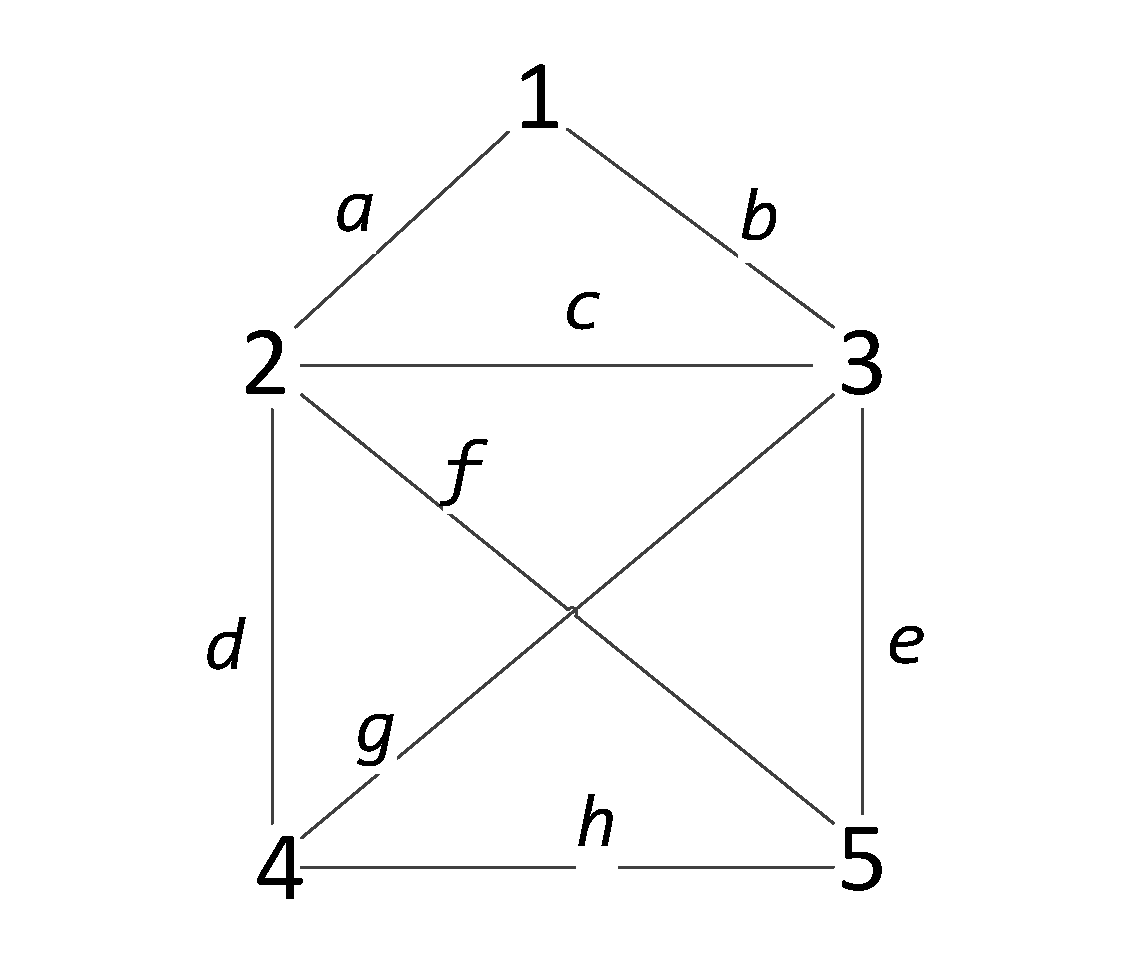
\includegraphics[scale=0.45]{envelope}
	\end{figure}

\end{frame}

\begin{frame}
	
	\frametitle{\insertsection}
	
	\begin{enumerate}
		\setcounter{enumi}{2}
		\item Даны два сосуда объемом 3 и 5 литров. Также имеется источник, из которого можно наполнить сосуды и куда можно вылить лишнюю воду.
		Определить последовательность переливаний, необходимую для получения 4 литров воды в одном из сосудов.
		\item Усовершенствовать решение предыдущей задачи таким образом, чтобы программа принимала на вход начальное состояние:
		целочисленные объемы сосудов V1 и V2, начальное количество воды в каждом сосуде и требуемое количество воды. При этом V1 и V2 взаимно просты.
		По начальному состоянию программа должна определить последовательность переливаний, необходимую для достижения целевого объема.
		Если задача не имеет решения~--- программа должна возвращать \texttt{false}.
	\end{enumerate}
	
\end{frame}


% Формальные грамматики (DCG)

\lecture{Definite clause grammars}{dcg}

\begin{frame}

	\begin{center}
		\Huge Понятие формальных грамматик
	\end{center}

\end{frame}

\section{Понятие формальных грамматик}
\subsection{Интуитивное определение}


\begin{frame}
	
	\frametitle{\insertsection}
	\framesubtitle{\insertsubsection}
	
	Одной из первых и основных областей применения Пролога является компьютерная лингвистика~--- обработка естественных языков
	автоматически. Формальная грамматика~--- это множество правил, которые определяют, какие фразы из заданного алфавита (лексикона)
	являются \textit{синтаксически корректными}. 
	
	Пролог предоставляет средства для описания подобных правил, а, следовательно, для
	задания грамматик, что позволяет проверить любую фразу на корректность относительно заданной грамматики, а также по грамматике 
	сгенерировать все возможные фразы, корректные относительно нее.
	
	Все фразы, синтаксически корректные относительно грамматики, называются \textbf{языком, порождаемым грамматикой}.
	
\end{frame}

\begin{frame}

	\frametitle{\insertsection}
	\framesubtitle{\insertsubsection}
	
	Контестно-свободная грамматика является частным случаем формальной грамматики.
	
	\begin{table}
		\centering
		\begin{tabular}{ l }
			\rowcolor{LightGray} sentense \(\rightarrow \) nounPhrase verbPhrase \\
			\rowcolor{LightGray} nounPhrase \(\rightarrow \) article noun \\
			\rowcolor{LightGray} verbPhrase \(\rightarrow \) verbExpr nounPhrase \\
			\rowcolor{LightGray} article \(\rightarrow \) a \\
			\rowcolor{LightGray} article \(\rightarrow \) the \\
			\rowcolor{LightGray} noun \(\rightarrow \) cat \\
			\rowcolor{LightGray} noun \(\rightarrow \) king \\
			\rowcolor{LightGray} verbExpr \(\rightarrow \) may look at
		\end{tabular}
	\end{table}

\end{frame}

\subsection{Дерево разбора}

\begin{frame}
	
	\frametitle{\insertsection}
	\framesubtitle{\insertsubsection}
	
	\begin{itemize}
		\item Данная грамматика содержит 8 правил.
		\item Символ \(\rightarrow \) означает переход в правиле: сущность из левой части правила можно разложить на составляющие таким образом, как указано
		в правой части.
		\item \texttt{sentence, nounPhrase, verbPhrase, article, noun, verbExpr}~--- нетерминальные символы (нетерминалы).
		\item \textit{a, the, cat, king, may look at}~--- терминальные символы (терминалы). Множество терминалов также называют \textbf{алфавитом} или \textbf{лексиконом}.
	\end{itemize}
	
\end{frame}

\begin{frame}

	\frametitle{\insertsection}
	\framesubtitle{\insertsubsection}
	
	Рассмотрим старую английскую поговорку \textit{A cat may look at a king}.
	
	\begin{figure}
		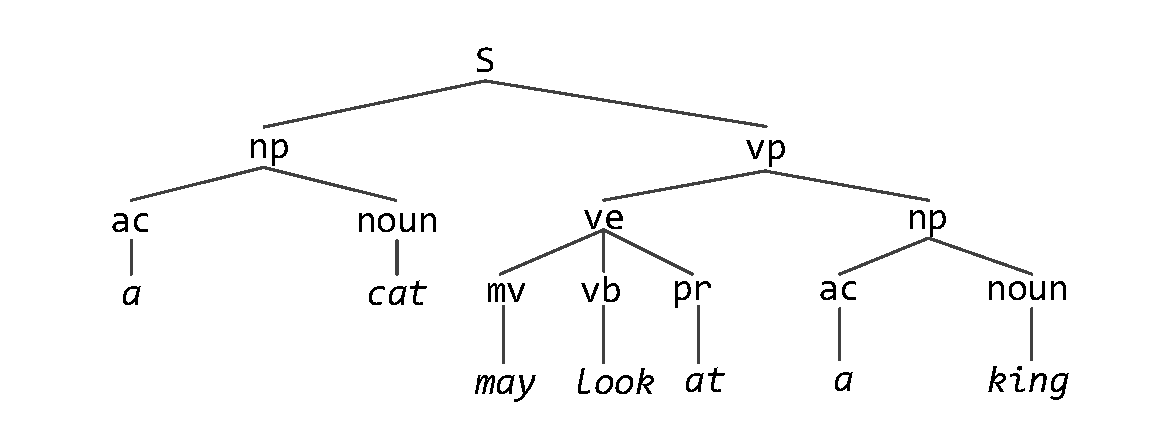
\includegraphics[scale=0.65]{gramtree}
	\end{figure}

\end{frame}


\begin{frame}

	\frametitle{\insertsection}
	\framesubtitle{\insertsubsection}
	
	Дерево разбора (parse tree) содержит информацию о синтаксической корректности и о структуре заданной фразы.
	
	\begin{enumerate}
		\item \textbf{Программа-распознаватель} (recognizer) по заданной строке сообщает, является ли эта строка синтаксически корректной относительно грамматики.
		\item \textbf{Программа-парсер} сообщает, является ли фраза синтаксически корректной и строит parse tree.
	\end{enumerate}

\end{frame}

\subsection{Контекстно-свободные языки}

\begin{frame}

	\frametitle{\insertsection}
	\framesubtitle{\insertsubsection}
	
	\begin{itemize}
		\item \textbf{Контекстно-свободным} называется язык, порождаемый контекстно-свободной грамматикой.
		\item Среди естественных языков контекстно-свободными являются, например, английский, фразцузский и немецкий языки.
		\item Многие языки программирования являются контекстно-свободными языками.
		\item Контекстно-свободные грамматики применяются при разработке компиляторов.
	\end{itemize}
	
\end{frame}

\begin{frame}

	\begin{center}
		\Huge Реализация КСГ на Прологе
	\end{center}

\end{frame}

\section{Реализация КСГ на Прологе}
\subsection{Recognizer}

\begin{frame}

	\frametitle{\insertsection}
	\framesubtitle{\insertsubsection}
	
	Сначала опишем грамматику.
	
	\texttt{\begin{itemize}
			\item[] sentense(S) :- nounPhrase(NP), verbPhrase(VP), append(NP,VP,S).
			\item[] nounPhrase(NP) :- article(A), noun(N), append(A,N,NP).
			\item[] verbPhrase(VP) :- verbExpr(VE), nounPhrase(NP), append(VE,NP,VP).
			\item[] verbExpr(VE) :- modalVerb(MV),verb(V),prep(P),append([MV,V,P],VE).
			\item[] article([A]) :- lexicon(''article'', A).
			\item[] noun([N]) :- lexicon(''noun'',N).
			\item[] modalVerb([MV]) :- lexicon(''modal verb'',MV).
			\item[] verb([V]) :- lexicon(''verb'',V).
			\item[] prep([P]) :- lexicon(''prep'',P).
	\end{itemize}}

\end{frame}


\begin{frame}

	\frametitle{\insertsection}
	\framesubtitle{\insertsubsection}
	
	Лексикон иногда выносят отдельно.
	
	\texttt{\begin{itemize}
			\item[] lexicon(''article``,''a``).
			\item[] lexicon(''article``,''the``).
			\item[] lexicon(''noun``,''cat``).
			\item[] lexicon(''noun``,''king``).
			\item[] lexicon(''verb``,''look``).
			\item[] lexicon(''modal verb``,''may``).
			\item[] lexicon(''prep``,''at``).
	\end{itemize}}

\end{frame}


\begin{frame}

	\frametitle{\insertsection}
	\framesubtitle{\insertsubsection}
	
	Два предиката для удобства запуска программы. Первый распознает введенную строку, отвечая \texttt{true} или \texttt{false}, а второй генерирует все
	фразы языка, порождаемого грамматикой.
	
	\texttt{\begin{itemize}
			\item[] recognize :- write(''Enter the phrase: ''),current\_input(In), read\_string(In, ''\textbackslash n'', ''\textbackslash r\textbackslash t'', \_, Phrase), split\_string(Phrase,~''~'',~"''',~ListPhrase), sentense(ListPhrase),!.
			\item[] generate :- sentense(Phrase), atomics\_to\_string(Phrase,'~',String),write(String).
	\end{itemize}}

\end{frame}

\begin{frame}

	\frametitle{\insertsection}
	\framesubtitle{\insertsubsection}
	
	Данная программа не будет эффективной.
	
	\begin{itemize}
		\item Она сначала пытается угадать фразу, а затем сравнивает ее с заданной.
		\item Вопрос \texttt{sentense([''a'',''cat'',''may'',''look'',''at'',''a'',''king''])} заставит программу проверять все возможные фразы до тех пор, пока очередная
		не совпадет с нужной.
		\item Причина в том, что в предикаты \texttt{nounPhrase, verbPhrase} и прочие поступают неопределенные переменные, которые требуют означивания.
		\item Это можно исправить, заставив программу сначала разбить фразу на части, а затем проверять эти части на соответствие правилам грамматики.
	\end{itemize}
	
	
\end{frame}


\begin{frame}

	\frametitle{\insertsection}
	\framesubtitle{\insertsubsection}
	
	
	В нашем случае это поможет при распознавании, но сломает генератор языка X\_X
	
	Кроме того, операция \texttt{append} очень дорогая и неэффективная.
	
	\texttt{\begin{itemize}
			\item[] sentense(S) :- append(NP,VP,S), nounPhrase(NP), verbPhrase(VP).
			\item[] nounPhrase(NP) :- append(A,N,NP), article(A), noun(N).
			\item[] verbPhrase(VP) :- append(VE,NP,VP), verbExpr(VE), nounPhrase(NP).
			\item[] verbExpr(VE) :- append([MV,V,P],VE), modalVerb(MV), verb(V), prep(P).
	\end{itemize}}


\end{frame}

\subsection{Разностные списки}


\begin{frame}

	\frametitle{\insertsection}
	\framesubtitle{\insertsubsection}
	
	\textbf{Разностный список} \texttt{L} представляется в виде двух списков \texttt{A} и \texttt{B} таких, что \texttt{L~=~A~\textbackslash~B}.
	Первый список в паре содержит то, что надо оставить, включить в список \texttt{L}, а второй~--- то, что следует отбросить из того, что мы включили.
	Один и тот же список можно представить в виде разностного списка бесконечным числом способов.
	
	\texttt{\begin{itemize}
			\item[] [a, cat, may, look, at, a, king] []
			\item[] [a, cat, may, look, at, a, king, wtf, omg] [wtf, omg]
	\end{itemize}}

\end{frame}


\begin{frame}

	\frametitle{\insertsection}
	\framesubtitle{\insertsubsection}
	
	Так будет выглядеть описание грамматики с разностными списками вместо \texttt{append}.
	
	\texttt{\begin{itemize}
			\item[] sentense(S,D) :- nounPhrase(S,VP), verbPhrase(VP,D).
			\item[] nounPhrase(NP,D) :- article(NP,N), noun(N,D).
			\item[] verbPhrase(VP,D) :- verbExpr(VP,VE), nounPhrase(VE,D).
			\item[] verbExpr(VE,D) :- modalVerb(VE,MV), verb(MV,V), prep(V,D).
			\item[] article([A|D],D) :- lexicon(''article'',A).
			\item[] noun([N|D],D) :- lexicon(''noun'',N).
			\item[] modalVerb([MV|D],D) :- lexicon(''modal verb'',MV).
			\item[] verb([V|D],D) :- lexicon(''verb'',V).
			\item[] prep([P|D],D) :- lexicon(''prep'',P).
	\end{itemize}}

\end{frame}

\subsection{Специальный синтаксис}


\begin{frame}

	\frametitle{\insertsection}
	\framesubtitle{\insertsubsection}
	
	Теперь рассмотрим, какие специальные средства предоставляет Prolog для описания грамматик.
	
	\texttt{\begin{itemize}
			\item[] sentense -{}-\textgreater~nounPhrase, verbPhrase.
			\item[] nounPhrase -{}-\textgreater~article, noun.
			\item[] verbPhrase -{}-\textgreater~verbExpr, nounPhrase.
			\item[] verbExpr -{}-\textgreater~modalVerb, verb, prep.
			\item[] article -{}-\textgreater~[''a''].
			\item[] article -{}-\textgreater~[''the''].
			\item[] noun -{}-\textgreater~[''cat''].
			\item[] noun -{}-\textgreater~[''king''].
			\item[] modalVerb -{}-\textgreater~[''may''].
			\item[] verb -{}-\textgreater~[''look''].
			\item[] prep -{}-\textgreater~[''at''].
	\end{itemize}}

\end{frame}


\begin{frame}

	\begin{center}
		\Huge Рекурсивные правила
	\end{center}

\end{frame}

\section{Рекурсивные правила}
\subsection{Что может пойти не так?}

\begin{frame}

	\frametitle{\insertsection}
	\framesubtitle{\insertsubsection}
	
	Допустим, мы хотим добавить соединительные правила для генерации бесконечных последовательностей утверждений.
	
	\begin{table}
		\centering
		\begin{tabular}{ l }
			\rowcolor{LightGray} sentense \(\rightarrow \) sentense conjunction sentense \\
			\rowcolor{LightGray} conjunction \(\rightarrow \) and \\
			\rowcolor{LightGray} conjunction \(\rightarrow \) or \\
			\rowcolor{LightGray} conjunction \(\rightarrow \) but \\
		\end{tabular}
	\end{table}
	

\end{frame}


\begin{frame}

	\frametitle{\insertsection}
	\framesubtitle{\insertsubsection}
	
	Нет ничего проще.
	
	\texttt{\begin{itemize}
			\item[] sentense -{}-\textgreater~sentense, conjunction, sentense.
			\item[] conjunction -{}-\textgreater~[''and''].
			\item[] conjunction -{}-\textgreater~[''or''].
			\item[] conjunction -{}-\textgreater~[''but''].
	\end{itemize}}

\end{frame}

\begin{frame}

	\frametitle{\insertsection}
	\framesubtitle{\insertsubsection}
	
	\begin{itemize}
		\item Если добавить рекурсивное правило в начало, то любой запрос на распознавание фразы приведет к бесконечному циклу и, как следствие, зависанию.
		Это произойдет потому, что в правиле первым стоит рекурсивный вызов. Любой запрос будет натыкаться на первое правило и бесконечно его применять.
		\item Если убрать рекурсивное правило в конец, то синтаксически правильные фразы будут распознаваться, но введение фразы, не являющейся верной в данной
		грамматике, опять-таки приведет к уходу в бесконечный цикл. На этот раз потому, что без возможности применить первое правило мы будем бесконечно пытаться применить второе.
		\item В случае обычной рекурсии такой эффект устраняется перестановкой рекурсивного вызова с первого места дальше. Но в случае грамматик последовательность
		предикатов в теле правила соответствует последовательности слов в синтаксически верных фразах, следовательно мы не можем менять предикаты местами.
	\end{itemize}

\end{frame}

\begin{frame}

	\frametitle{\insertsection}
	\framesubtitle{\insertsubsection}
	
	Так что же делать?
	
	\texttt{\begin{itemize}
			\item[] plainSentense -{}-\textgreater~nounPhrase, verbPhrase.
			\item[] sentense -{}-\textgreater~plainSentense.
			\item[] sentense -{}-\textgreater~plainSentense, conjunction, sentense.
	\end{itemize}}

\end{frame}

\subsection{Формальные языки}

\begin{frame}

	\frametitle{\insertsection}
	\framesubtitle{\insertsubsection}
	
	Рассмотрим формальный язык \(a^nb^n \). Все слова данного языка состоят из двух последовательностей из равного количества букв \(a\) и \(b\),
	идущих друг за другом. Пустое слово также является словом данного языка.
	
	\only<2->{\texttt{\begin{itemize}
			\item[] s --> [].
			\item[] s --> [a],s,[b].
	\end{itemize}}}

\end{frame}

\begin{frame}

	\begin{center}
		\Huge Упражнения
	\end{center}

\end{frame}


\section{Упражнения}

\begin{frame}

	\frametitle{\insertsection}

	\begin{enumerate}
		\item Реализуйте грамматику для языка \(a^nb^n - \{\mathcal{E} \}\).
		\item Реализуйте грамматику для языка \(a^nb^{2m}c^{2m}d^n \).
	\end{enumerate}
	

\end{frame}

\section{Задачи для самостоятельной работы}

\begin{frame}

	\begin{center}
		\Huge \insertsection
	\end{center}

\end{frame}

\begin{frame}

\frametitle{\insertsection}

	Реализовать контекстно-свободную грамматику для проверки корректности S-выражений в языке Clojure.
	Будем рассматривать лишь подмножество его синтаксиса, исключив специфические компоненты.
	
	Основа синтаксиса определяется следующим образом:
	
	\begin{enumerate}
		\item \textbf{Разделитель}. Пробел, табуляция, конец строки, запятая.
		\item \textbf{Атом}.
		\begin{enumerate}
			\item Число. Ограничимся целыми.
			\item Строка. Любая последовательность символов в двойных кавычках.
			\item Идентификатор. Либо последовательность букв, цифр и спецсимволов, начинающаяся с буквы, либо последовательность спецсимволов. Например
			\alert{-\textgreater} является валидным идентификатором. Можно ограничиться спецсимволами \alert{+, -, \textgreater, <, =}.
			\item Ключевые слова. Ключевое слово~--- это идентификатор, предваряемый двоеточием. Например \alert{:Num, :x, :Identifier}.
		\end{enumerate}
		\item \textbf{S-выражение}.
	\end{enumerate}

\end{frame}


\begin{frame}

\frametitle{\insertsection}

	S-выражение рекурсивно строится из атомов, разделителей и скобок.
	
	\begin{itemize}
		\item Любой атом является S-выражением.
		\item Последовательность S-выражений, разделенных разделителями и заключенная в круглые скобки, является S-выражением.
		\textbf{(S1 S2 S3,S4)}.
		\item Последовательность S-выражений, разделенных разделителями и заключенная в квадратные скобки, является S-выражением.
		\textbf{[S1 S2 S3 S4]}.
		\item Последовательность из четного числа S-выражений, разделенных разделителями и заключенная в фигурные скобки, является S-выражением.
		\textbf{\{S1 S2 S3 S4\}}.
	\end{itemize}

\end{frame}


\begin{frame}

\frametitle{\insertsection}

	Программа должна принимать S-выражение, записанное в виде строки, и отвечать \texttt{true} в случае, когда выражение корректно относительно синтаксиса
	языка Clojure, и \texttt{false} в противном случае.
	
	\begin{rexample}
		s\_expression(''(inc 1)``). \\
		s\_expression(''(+ [x y])``). \\
		s\_expression(''((lambda x (nth [(tail x) 0])) (list \textbackslash''Some string\textbackslash``))``).\\
		s\_expression(''\{list (-> A (:List A)),nth (-> (cross (:List A) :Num) (:List A)), tail (-> (:List A)  (:List A))\}``).
	\end{rexample}

\end{frame}